\section{progettazione concettuale}
\subsection{Introduzione}
Il modello concettuale rappresenta la struttura logica del database, definendo le entità, gli attributi e le relazioni tra di esse. In questa fase, si è proceduto a identificare le principali entità del sistema e a stabilire le relazioni che le collegano, garantendo così una visione chiara e coerente delle informazioni da gestire.
\subsection{UML non ristrutturato}
\begin{figure}[H]
    \noindent\makebox[\linewidth]{%
        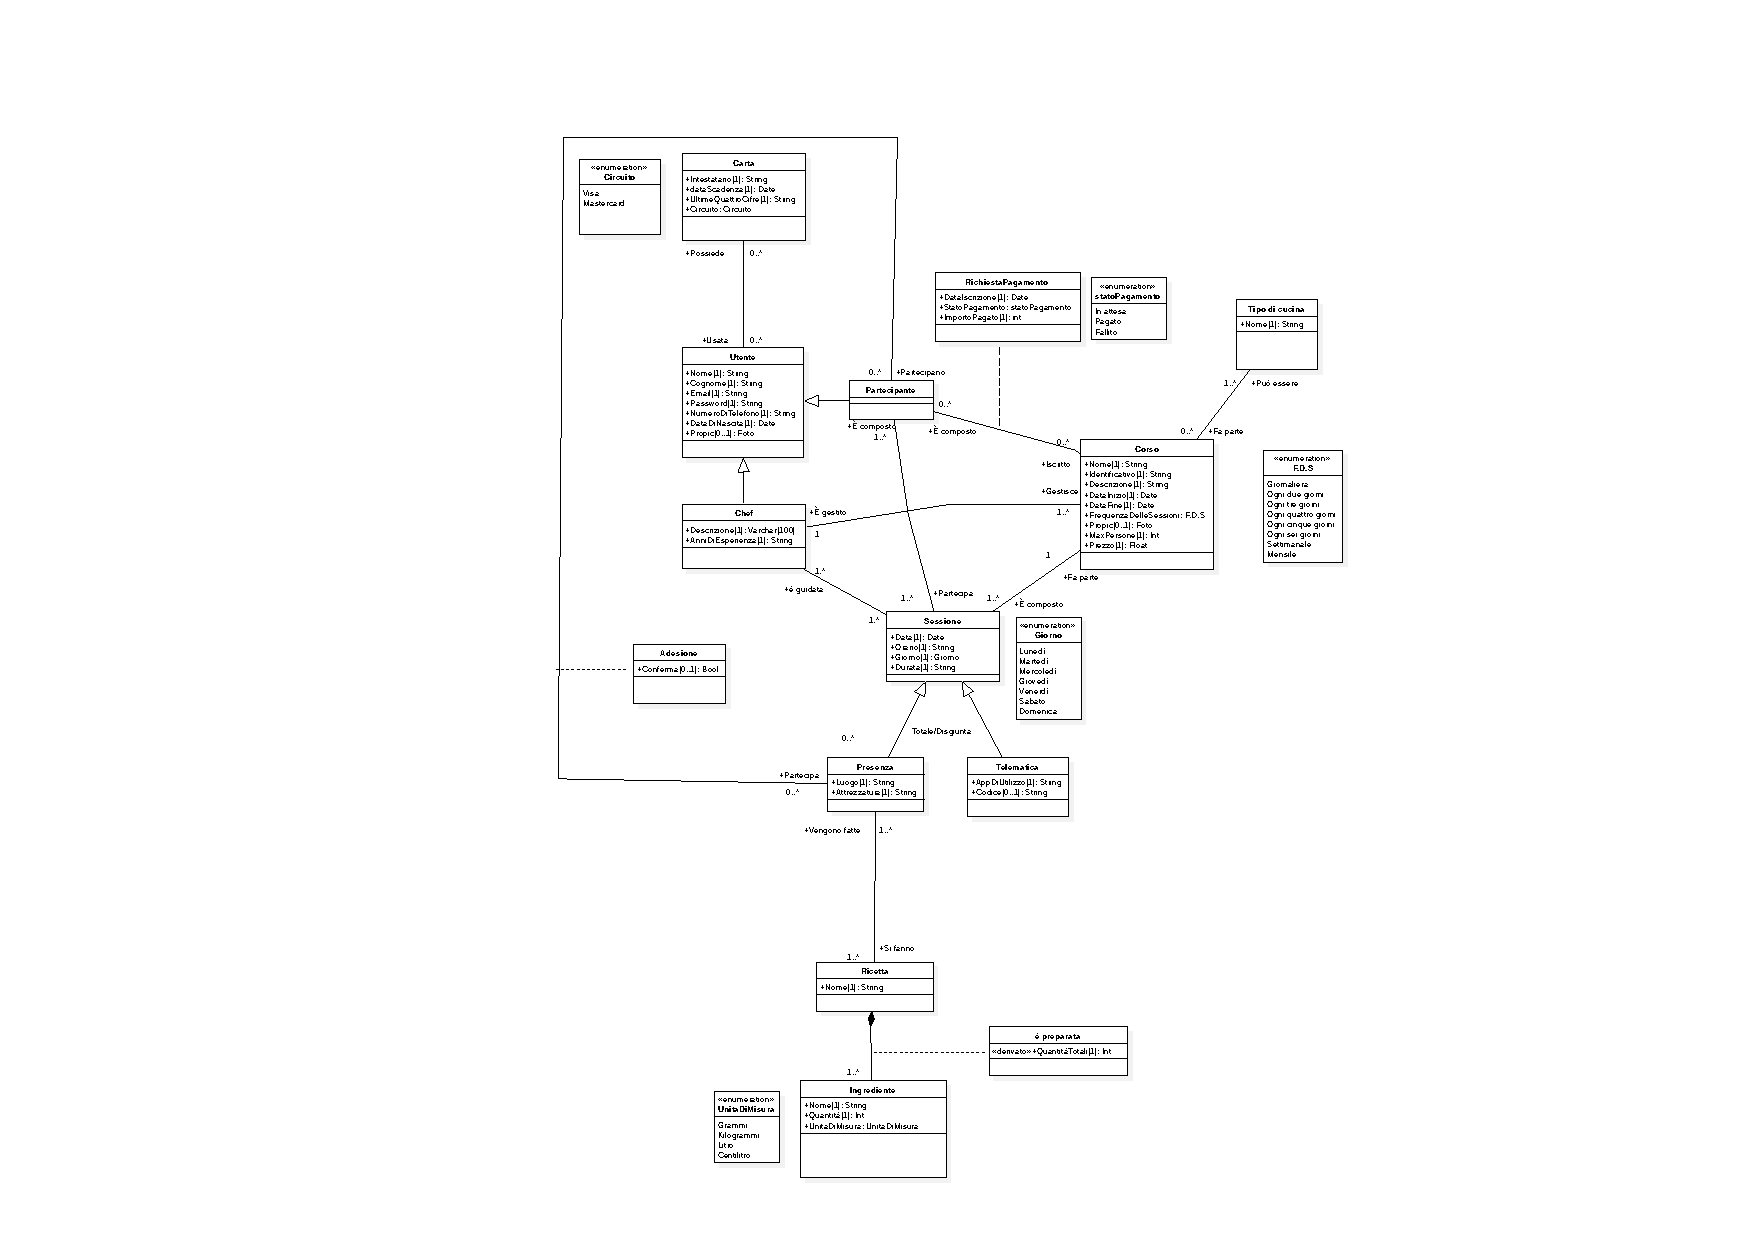
\includegraphics[height=0.9\textheight,width=2\textwidth]{latex/immagini/uml_non_ristrutturato.pdf}
    }
    \caption{Diagramma UML del sistema}
\end{figure}
\subsubsection{Entità principali}
Le entità principali identificate nel sistema sono:
\begin{itemize}
    \item \textbf{Utente}: L’utente rappresenta il soggetto fruitore del sistema, che può iscriversi ai corsi e partecipare alle sessioni. I principali attributi includono nome, cognome, email, password, data di nascita e una foto di profilo. Ogni utente può essere associato a una o più carte di pagamento e può diventare partecipante a diversi corsi.
    \item \textbf{Chef}: Lo chef è un utente con il ruolo specifico di organizzare corsi. Ogni chef dispone di una descrizione e di un numero di anni di esperienza. Un chef può gestire più corsi, ma ogni corso è gestito da un solo chef.
    \item \textbf{Corso}: Il corso è l'entità centrale del sistema e rappresenta una proposta didattica su un tema gastronomico specifico. Contiene attributi quali nome, descrizione, identificativo, data di inizio/fine, frequenza delle sessioni, prezzo, massimo persone che possono iscriversi, immagine di copertina e tipo di cucina (gestito da un'altra entità). Ogni corso è composto da più sessioni e prevede una relazione molti-a-molti con i partecipanti.
    \item \textbf{Sessione}: Ogni corso è articolato in una o più sessioni, ciascuna delle quali ha una data, un orario, un insieme di giorni della settimana in cui si svolge, e una durata. Le sessioni sono specializzate in due sottotipi mutuamente esclusivi:
    \begin{itemize}
        \item \textbf{Presenza}: Con attributi come luogo e attrezzature richieste.
        \item \textbf{Telematica}: Con attributi relativi all'app utilizzata e al codice di accesso.
    \end{itemize}
    \item \textbf{Partecipante e Adesione}: La partecipazione ai corsi è modellata tramite l’entità Partecipante, che collega utenti e corsi. La partecipazione a sessioni pratiche richiede un’adesione esplicita, rappresentata dall'entità Adesione, che contiene un attributo booleano di conferma.
    \item \textbf{Ricetta e Ingredientemento}: Ogni sessione pratica può includere la preparazione di una o più ricette. Ogni ricetta è composta da uno o più ingredienti, ciascuno dei quali ha un nome, e un'unità di misura (enumerata). La relazione tra Ricetta e Ingrediente è associativa e include l'attributo QuantitàTotale e QuantitàUnitaria, utile per calcolare la quantità necessaria in base alle adesioni.
    \item \textbf{Carta e RichiestaPagamento}: Gli utenti possono associare al proprio profilo una o più carte di pagamento, appartenenti a un circuito specificato tramite enumerazione (Visa, Mastercard). Le richieste di pagamento sono entità separate, con data, stato (in attesa, pagato, fallito) e importo.
\end{itemize}
\subsubsection{Gerarchie e generalizzazioni}
Nel modello concettuale, sono state identificate le seguenti gerarchie e generalizzazioni:
\begin{itemize}
    \item \textbf{Sessione}: Le sessioni sono suddivise in due sottotipi: \textit{Presenza} e \textit{Telematica}. Questa specializzazione consente di gestire le specificità di ciascun tipo di sessione, come il luogo e le attrezzature per le sessioni in presenza, e l'app utilizzata e il codice di accesso per quelle telematiche.
    \item \textbf{Utente}: L'entità Utente può essere specializzata in due sottotipi: \textit{Partecipante} e \textit{Chef}. Questa distinzione permette di gestire le diverse funzionalità e attributi associati a ciascun ruolo nel sistema.
\end{itemize}
Entrambe le specializzazioni sono totali e disgiunte, di conseguenza ogni istanza di Sessione sia esclusivamente di uno dei due tipi e che ogni Utente sia o un Partecipante o uno Chef, ma non entrambi contemporaneamente.
\subsubsection{Relazioni tra le entità}
Le relazioni tra le entità sono state definite come segue:
\begin{itemize}
    \item \textbf{Utente - Partecipante}: Un utente può essere un partecipante a più corsi, e ogni corso può avere più partecipanti. Questa relazione è molti-a-molti.
    \item \textbf{Chef - Corso}: Ogni chef può gestire più corsi, ma ogni corso è associato a un solo chef. Questa relazione è uno-a-molti.
    \item \textbf{Corso - Sessione}: Un corso può avere più sessioni, ma ogni sessione appartiene a un solo corso. Questa relazione è uno-a-molti.
    \item \textbf{Sessione - Partecipante}: Ogni partecipante può aderire a più sessioni pratiche, e ogni sessione può avere più partecipanti. Questa relazione è molti-a-molti, mediata dall'entità Adesione.
    \item \textbf{Corso - Ricetta}: Ogni corso può includere più ricette, e ogni ricetta può essere associata a più corsi. Questa relazione è molti-a-molti.
    \item \textbf{Ricetta - Ingrediente}: Ogni ricetta può includere più ingredienti, e ogni ingrediente può essere utilizzato in più ricette. Questa relazione è molti-a-molti, mediata dall'attributo QuantitàTotale.
    \item \textbf{Utente - Carta}: Un utente può avere più carte di pagamento associate al proprio profilo. Questa relazione è uno-a-molti.
    \item \textbf{Ricetta - Ingrediente}: Ogni ricetta può essere associata a più ingredienti, e ogni ingrediente può essere utilizzato in più ricette. Questa relazione è una composizione, mediata dall'attributo QuantitàTotale.
\end{itemize}
\subsubsection{Motivazione delle scelte progettuali}
Le scelte progettuali sono state guidate dalla necessità di garantire una rappresentazione chiara e coerente delle informazioni, facilitando la gestione dei corsi, delle sessioni e delle partecipazioni. La specializzazione delle sessioni in Presenza e Telematica consente di gestire le specificità di ciascun tipo di sessione, mentre la distinzione tra Partecipante e Chef permette di differenziare i ruoli degli utenti nel sistema. Inoltre, l'uso di relazioni molti-a-molti per gestire le adesioni alle sessioni pratiche e le associazioni tra ricette e ingredienti garantisce flessibilità e scalabilità nel modello.
\subsection{UML ristrutturato}
\begin{figure}[H]
    \noindent\makebox[\linewidth]{%
        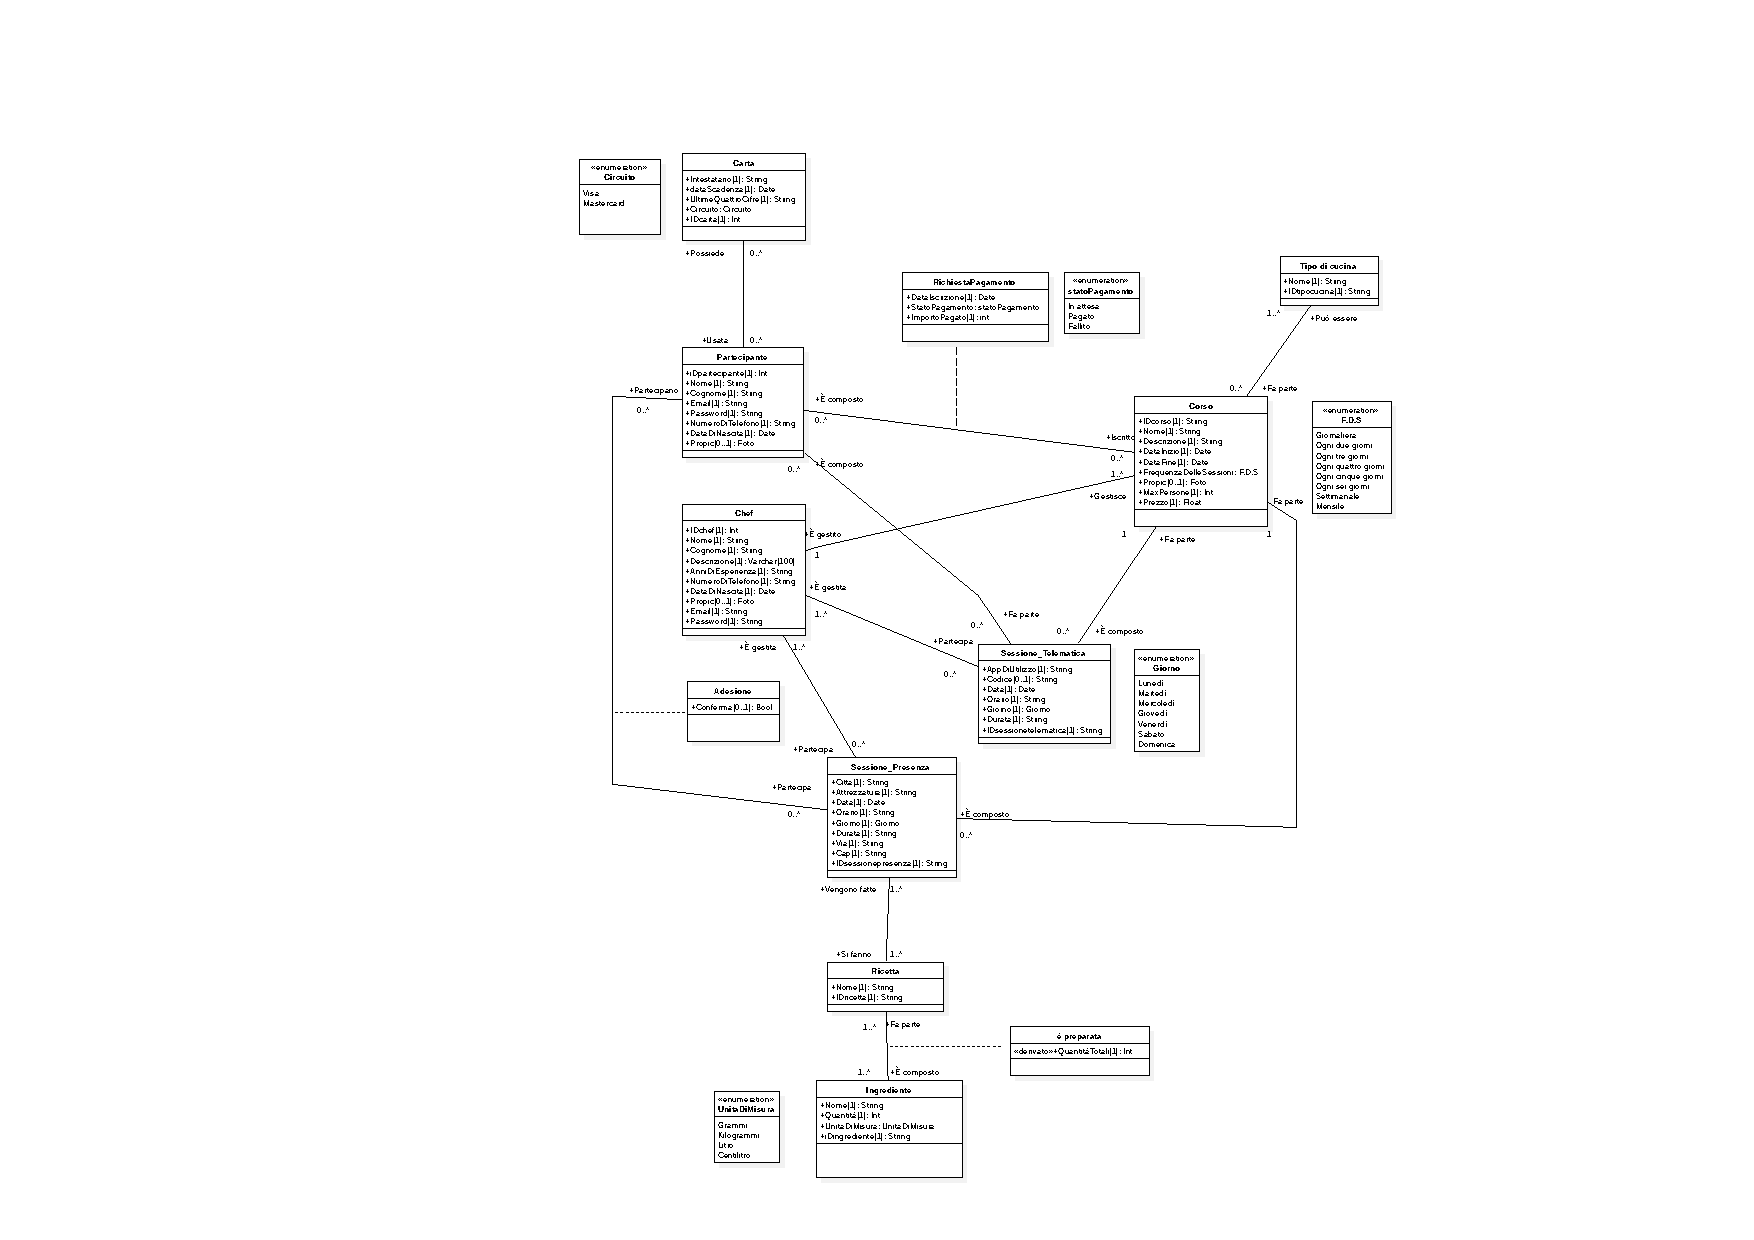
\includegraphics[height=0.9\textheight,width=2\textwidth]{latex/immagini/uml_ristrutturato.pdf}
    }
    \caption{Diagramma UML ristrutturato del sistema}
\end{figure}
\subsubsection{Modifiche rispetto al modello non ristrutturato}
Il modello ristrutturato presenta alcune modifiche rispetto al modello non ristrutturato, adattandolo a un database relazionale. Le principali modifiche includono:
\begin{itemize}
    \item \textbf{Rimozione delle gerarchie}: Le gerarchie tra le entità sono state rimosse, trasformando le specializzazioni in entità separate. Ad esempio, le sessioni di tipo Presenza e Telematica sono state trasformate in due entità distinte, mantenendo gli attributi specifici per ciascun tipo.
    \item \textbf{Attributi composti e multivalore}: Gli attributi composti e multivalore sono stati normalizzati. Ad esempio, l'attributo \textit{Luogo} è stato suddiviso in attributi separati per \textit{Città}, \textit{Indirizzo} e \textit{Cap}.
    \item \textbf{Aggiunta di chiavi primarie e esterne}: Ogni entità ha una chiave primaria univoca, e le relazioni tra le entità sono definite tramite chiavi esterne, garantendo l'integrità referenziale del database.
\end{itemize}

\subsubsection{Comportamento del modello ristrutturato con le modifiche}
Il modello ristrutturato mantiene le proprietà di specializzazione totale e disgiunta, adattandosi alle modifiche apportate. In particolare:
\begin{itemize}
    \item \textbf{Specializzazione totale e disgiunta}: Le entità separate per le sessioni di tipo Presenza e Telematica garantiscono che ogni sessione appartenga esclusivamente a uno dei due tipi, rispettando la disgiunzione. Inoltre, ogni utente è classificato come Partecipante o Chef, assicurando che la specializzazione sia totale e disgiunta.
    \item \textbf{Integrità referenziale}: L'uso di chiavi primarie, esterne e l'aggiunta di chiavi surrogate garantisce che le relazioni tra le entità siano coerenti e che non si verifichino violazioni di integrità nel database.
\end{itemize}

\subsubsection{Motivazioni delle scelte del modello ristrutturato}
Le motivazioni alla base delle scelte progettuali del modello ristrutturato derivano dalla necessità di garantire una rappresentazione chiara, coerente e scalabile delle informazioni, adattandosi alle esigenze di un database relazionale. Una delle principali considerazioni riguarda la gestione delle specializzazioni totali e disgiunte, che hanno permesso di semplificare il modello concettuale senza perdere la coerenza logica.

Nel modello ristrutturato, le specializzazioni totali e disgiunte sono state gestite trasformando la classe generale in entità separate per ciascuna specializzazione. Questo approccio consente di incorporare gli attributi della classe generale direttamente nelle entità specializzate, eliminando la necessità di mantenere una gerarchia tra le entità. Ad esempio, nel caso delle sessioni, la classe generale "\textbf{Sessione}" è stata suddivisa in due entità distinte: "\textbf{Sessione\_Presenza}" e "\textbf{Sessione\_Telematica}". Ogni entità specializzata include gli attributi specifici del proprio tipo, come il luogo e le attrezzature richieste per le sessioni in presenza, e l'app utilizzata e il codice di accesso per quelle telematiche. In questo modo, si garantisce che ogni sessione appartenga esclusivamente a uno dei due tipi, rispettando la disgiunzione, e che tutte le sessioni siano rappresentate nel modello, rispettando la totalità, facilitando anche le associazioni tra le varie entità.

La stessa logica è stata applicata alla specializzazione dell'entità "Utente", suddivisa in "Partecipante" e "Chef". Ogni utente è classificato come Partecipante o Chef, ma non può appartenere a entrambe le categorie contemporaneamente. Gli attributi comuni agli utenti, come nome, cognome, email e data di nascita, sono stati incorporati direttamente nelle entità specializzate, mentre gli attributi specifici, come la descrizione e gli anni di esperienza per gli Chef, sono stati aggiunti solo alla rispettiva entità. Questo approccio semplifica la gestione delle entità nel database, eliminando la necessità di un'entità generale "Utente" e garantendo che la specializzazione rimanga totale e disgiunta.

Per quanto riguarda le associazioni tra le entità, il modello ristrutturato utilizza chiavi primarie e chiavi esterne per definire le relazioni, garantendo l'integrità referenziale del database. Ad esempio, la relazione tra "Corso" e "Sessione" è uno-a-molti, con l'identificativo del corso utilizzato come chiave esterna nelle entità "Presenza" e "Telematica". Questo approccio consente di mantenere la coerenza delle informazioni e di semplificare le operazioni di query e aggiornamento. Analogamente, la relazione molti-a-molti tra "Sessione" e "Partecipante" è mediata dall'entità "Adesione", che include un attributo booleano di conferma per gestire la partecipazione alle sessioni pratiche.

Un altro esempio significativo riguarda la relazione tra "Ricetta" e "Ingrediente". Nel modello ristrutturato, questa relazione è stata normalizzata utilizzando un'entità associativa che include l'attributo "QuantitàTotale". Questo approccio consente di calcolare facilmente la quantità necessaria di ciascun ingrediente in base alle adesioni alle sessioni pratiche, garantendo flessibilità e scalabilità nel modello.
\begin{figure}[H]
    \noindent\makebox[\linewidth]{
        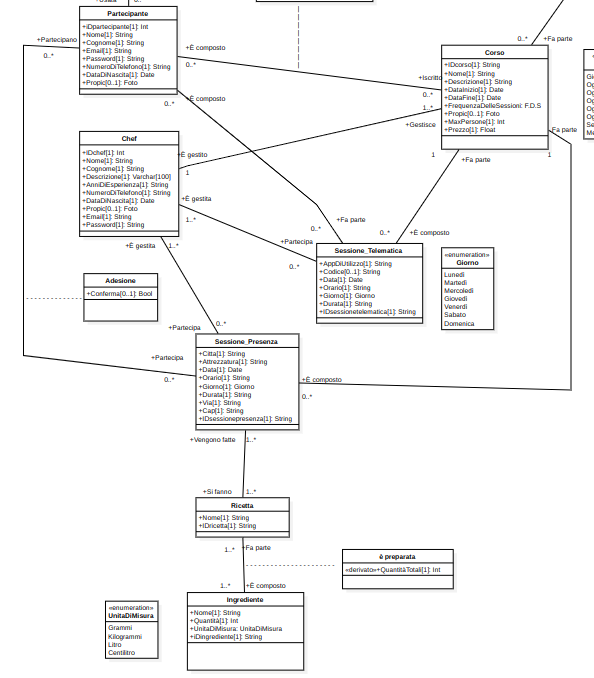
\includegraphics[height=0.8\textheight,width=1\textwidth]{latex/immagini/uml_ristrutturato_sessioni.png}
    }
    \caption{Scelte ristrutturato}
\end{figure}